\documentclass[../probability-notes.tex]{subfiles}
\begin{document}
    %%%%%%%%%%%%%%%%%%%%%%%%%%%%%%%%%%%%%%%%%%%%%%%%%%%%%%%%%%%%%%%%%%%%%%%%%%%
    \section{t-Distribution}
    Let $Z$ be a standard normal random variable and let $\chi_{n}^{2}$ be a chi-square random variable. Assuming these two random variables are independent, the radom variable $T_{n}$ is
    \begin{align*}
        T_{n} = \frac{Z}{\sqrt{\chi_{n}^{2}/n}}
    \end{align*}
    is said to have a t-distribution with $n$ degrees of freedom.\newline
    This distribution is symmetric around the normal, and as $n$ increases, the distribution becomes more and more like the standard normal distribution.

    \begin{figure}[h]
    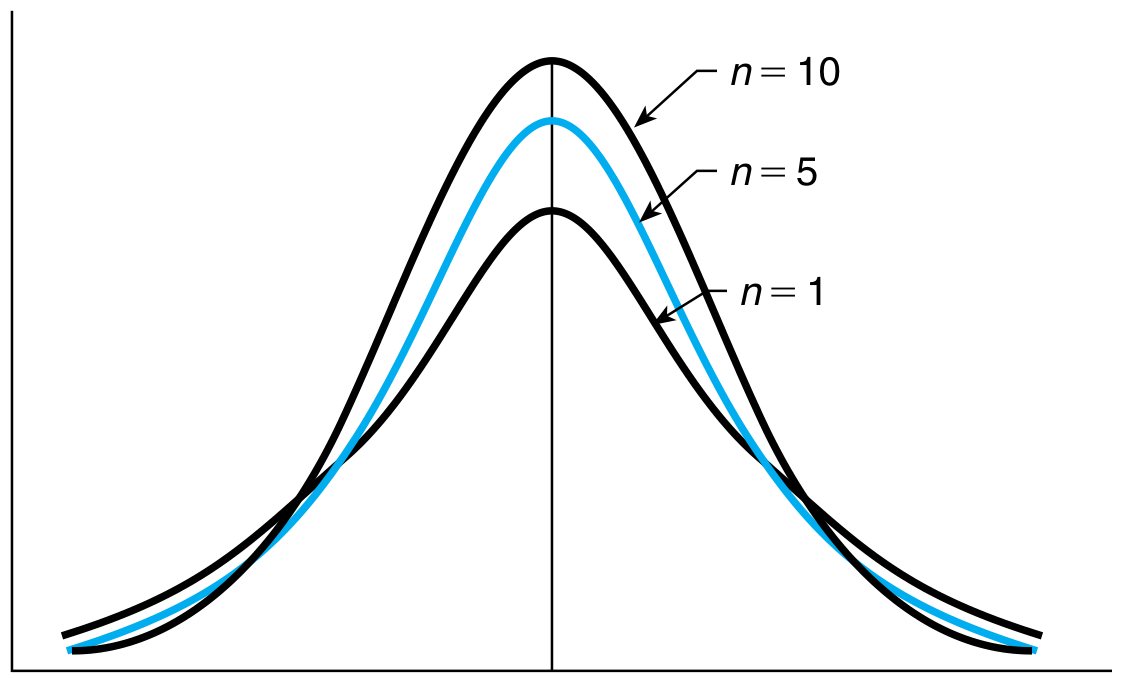
\includegraphics[scale=0.25]{t_1}
    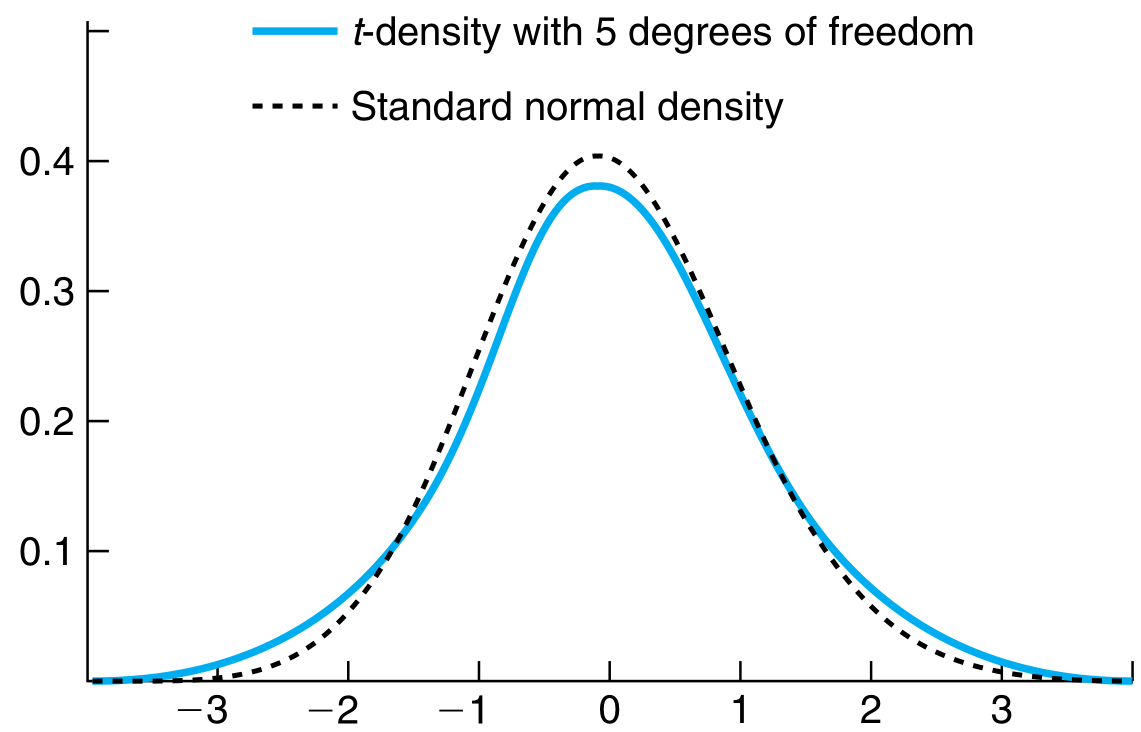
\includegraphics[scale=0.25]{t_2}
    \centering
    \caption{t-distribution for different degrees of freedom, and comparison with standard normal}
    \label{fig:t_1} %\ref{fig:t_1}
    \end{figure}

    From figure \ref{fig:t_1}, we see that t-distribution is heavier tailed than a standard normal. Translation, this means that a larger value is more likely to occur under a t-distribution than a standard normal. Furthermore, the heavy tails imply more variance than the standard normal.\newline

    For $\alpha between 0$ and $1$, let $t_{\alpha, n}$ be such that
    \begin{align*}
        P(T_{n} \geq t_{\alpha, n}) = \alpha
    \end{align*}
    By symmetry around the origin,
    \begin{align*}
        P(T_{n} \leq -t_{\alpha, n}) &= \alpha\\
        \text{or, \;} P(T_{n} \geq -t_{\alpha, n}) &= 1 - \alpha\\
        \text{and, \;} -t_{\alpha, n} &= t_{1 - \alpha, n}
    \end{align*}

    These standard values are available in math charts since they form the basis of the t test.

    \begin{figure}[h]
    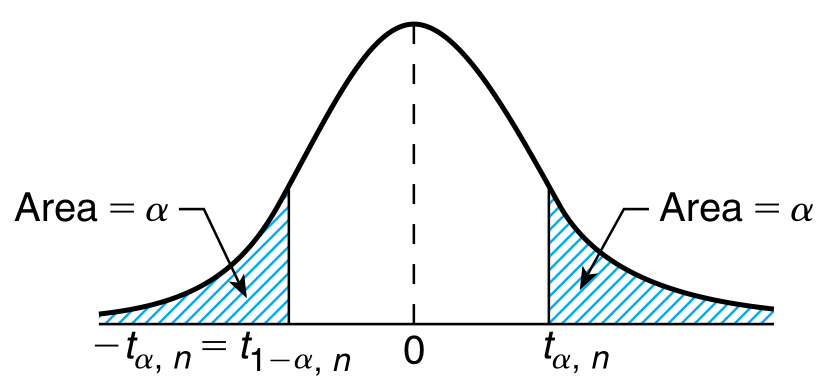
\includegraphics[scale=0.4]{t_3}
    \centering
    \caption{visual representation of $t_{\alpha,n}$}
    \label{fig:t_2} %\ref{fig:t_2}
    \end{figure}

    %%%%%%%%%%%%%%%%%%%%%%%%%%%%%%%%%%%%%%%%%%%%%%%%%%%%%%%%%%%%%%%%%%%%%%%%%%%
    \subsection{Mean and Variance}
    The following are stated without proof
    \begin{align*}
        \Aboxed{E[T_{n}] &= 0}\\
        \Aboxed{Var(T_{n}) &= \frac{n}{n-2}}\\
    \end{align*}

    In the limit of large $n$, the variance is close to $1$, which is consistent with the fact that the distribution resembles a standard normal in that limit.

\end{document}